\section{Software (Sistema integrado)}

    Como dito anteriormente, os dados 
    dos sensores serão transmitidos para um banco de dados,
    nesse deverá ser gravado os dados dos sensores:
    as temperaturas minimas e máximas, também as temperaturas 
    padrão a cada 10 segundos, essa frequência de 
    escrita de temperatura no banco poderá ser alterado caso o 
    cliente assim deseje.

    Sobre a nuvem, ela deverá ser feita preferencialmente 
    em Kubernetes para poder facilmente gerenciar todos os containers 
    de cada parte da aplicação de forma isolada, e além disso 
    poder integrar e instalar o sistema em diferentes nuvens
    e alternar entre elas de forma simples e rápida, 
    proporcionando assim maior estabilidade e disponibilidade
    aos serviços do sistema.

    \begin{citacao}[english]
        (...)
        Kubernetes aims to simplify the deployment and management 
        of services, including the construction of applications 
        as sets of interacting but independent services.
        (...)
        \cite{brewer2015kubernetes}
    \end{citacao}

    Sobre as linguagens e ferramentas que serão utilizadas
    no sistema, o front-end será feito usando o framework 
    de JavaScript React e o back-end será feito em PHP 8
    uma linguagem simples, poderosa e rápida, que irá se comunicar
    com o banco de dados que deverá ser relacional e com recursos
    para alta disponibilidade, para a escolha do banco pensando nos
    critérios anteriores e em um custo baixo foi escolhido o 
    PostgreSQL.

    A integração entre o back-end e o front-end será feita 
    através de uma API REST, o que possibilita a integração 
    com varias interfaces diferentes, e até entre diferentes
    sistemas caso necessário, essa API também será usada 
    para conectar os microcontroladores com o banco de dados.

    O sistema será primariamente acessado pelo computador
    utilizando um navegador web, como Google Chrome, 
    Opera, Firefox, etc. 
    Porem devido a responsividade do sistema também será
    possível acessá-lo pelo navegador de um smartphone,
    caso o cliente tenha interesse no desenvolvimento de
    um aplicativo para smartphones android e IOS
    poderemos criar esse aplicativo utilizando 
    React Native, claro que o desenvolvimento do aplicativo
    adicionará um investimento maior ao projeto.


    % Quanto a mobilidade do sistema, como é um sistema web
    % então é acessado pelo navegador e pode ser facilmente
    % acessado por um SmartPhone, o sistema será responsivo,
    % porem se o cliente quiser um desempenho melhor e
    % uma experiencia personalizada, um aplicativo
    % mobile pode ser desenvolvido em React Native
    % juntamente como o sistema, claro que isso aumentará
    % os custos do desenvolvimento.
%
    % Sobre o sistema em si no quesito interface e funcionalidades
    % como é possível visualizar na figura \ref{fig:sistemaHome}
    % o sistema terá um design flat, limpo e direto com fundo e
    % tons mais escuros para não cansar a vista dos usuários que
    % responsáveis pelo monitoramento de temperatura das vacinas,
    % contará também com a opção de alterar a temperatura ideal,
    % de atenção e de alerta dos freezeres.
%
    % Sobre as funcionalidades do sistema em si, ele terá um
    % fundo escuro para não cansar as vistas dos usuários,
    % o sistema também possibilitará a mudança da temperatura
    % ideal, de atenção e alerta caso necessário,
%
    % O sistema também contará com telas para visualizar todo
    % o histórico das variações de temperaturas,
    % como também será possível visualizar a temperatura
    % das vacinas em tempo real, como mostrado nas figuras
    % \ref{fig:sistemaHistorico} e \ref{fig:sistemaTempReal}.

    O software terá primariamente uma tela inicial 
    como podem observar na figura \ref{fig:desktopHome}, 
    onde será possível navegar para as outras telas;
    que serão as telas de configuração dos limites
    de temperatura como mostrado na 
    figura \ref{fig:desktopConfigTemp};
    além de ter acesso a dashboards mostrando 
    mínimos, máximos e a temperatura atual 
    como é possível observar nas figuras 
    \ref{fig:desktopDashboard1} e \ref{fig:desktopDashboard2};
    e finalmente as visualizações de temperatura em 
    tempo real (figura \ref{fig:desktopTempAtual})
    e os históricos de variações de temperaturas,
    figuras \ref{fig:desktopTempDiaria} e \ref{fig:desktopTempSemanal}
    respectivamente.

    \begin{figure}
        \caption{Layout desktop home}
        \centering
        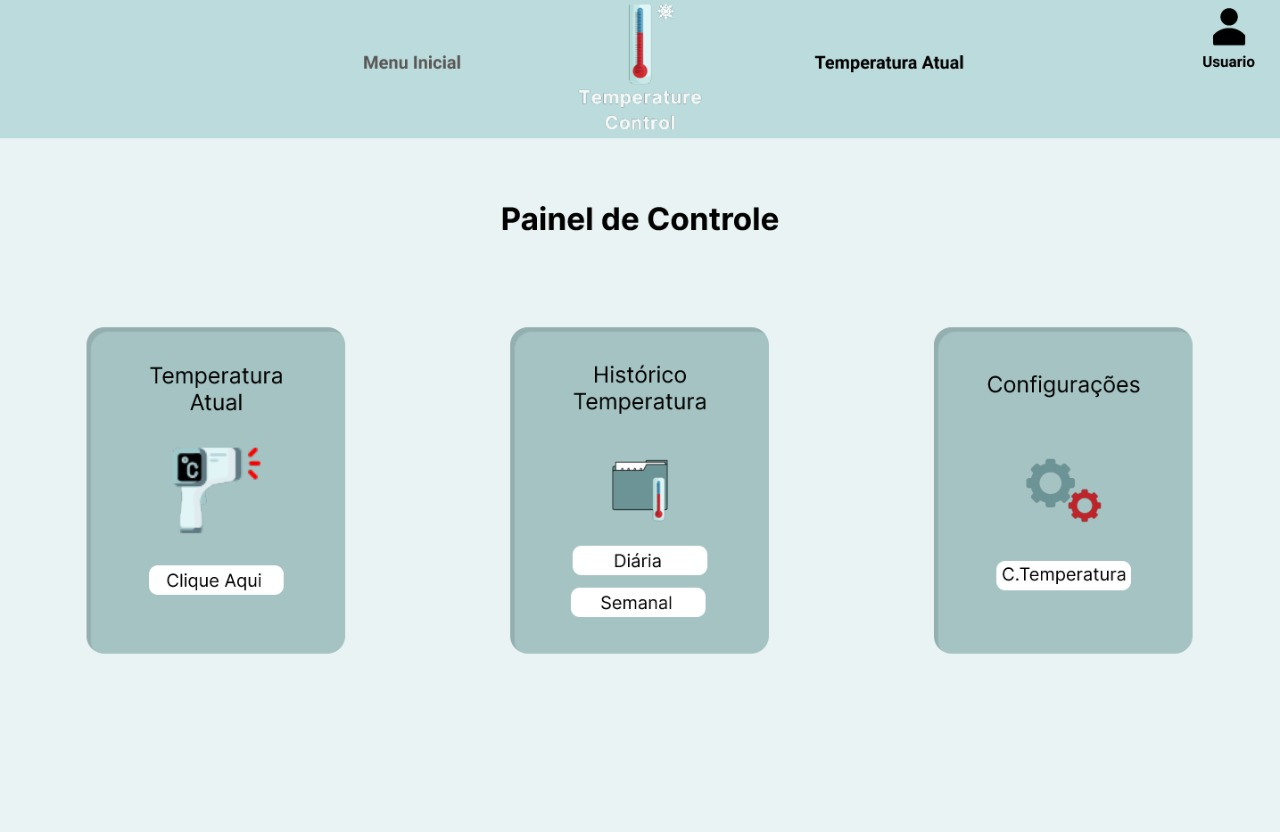
\includegraphics[scale=0.35]{img/desktop/home.jpeg}
        \legend{Fonte: Elaborado pelos autores}
        \label{fig:desktopHome}
    \end{figure}
    \begin{figure}
        \caption{Layout desktop configuração de temperatura}
        \centering
        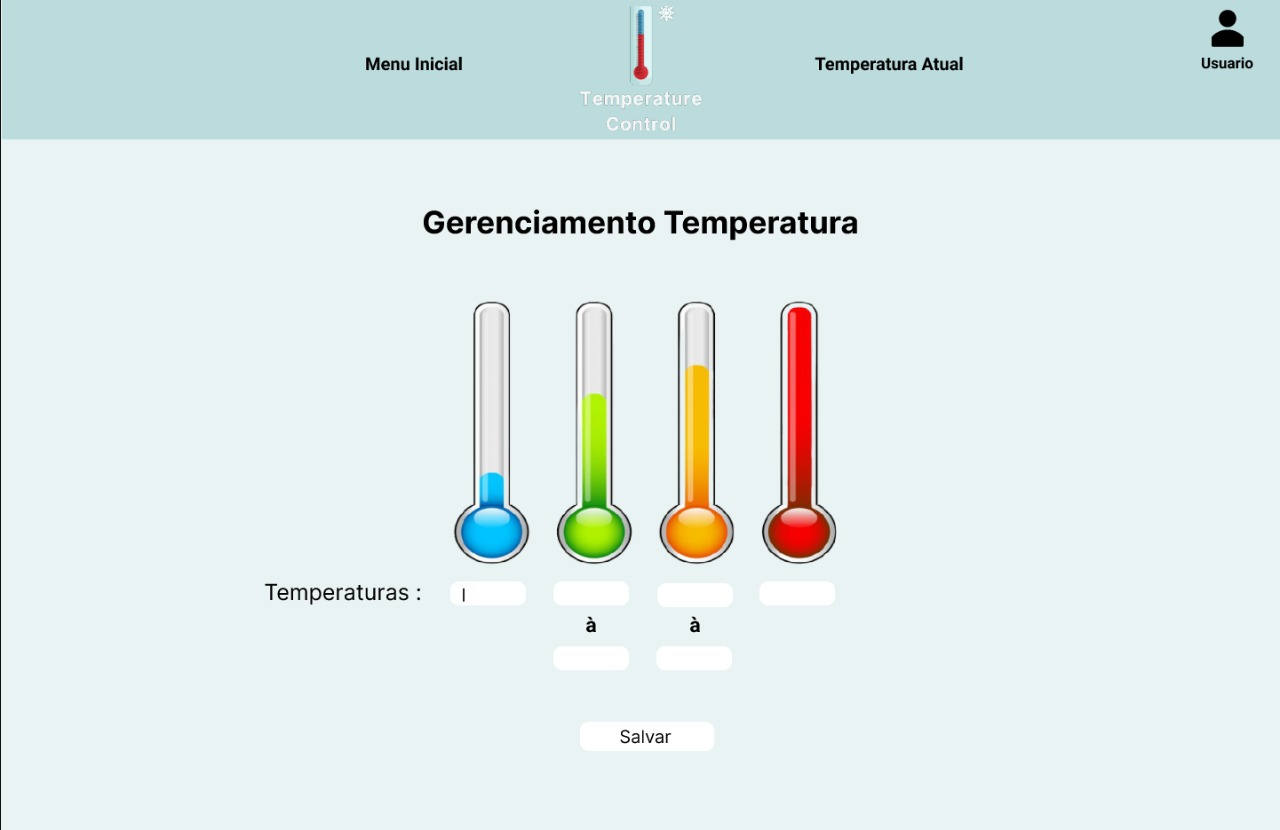
\includegraphics[scale=0.35]{img/desktop/config_temp.jpeg}
        \legend{Fonte: Elaborado pelos autores}
        \label{fig:desktopConfigTemp}
    \end{figure}
    \begin{figure}
        \caption{Layout desktop temperatura atual}
        \centering
        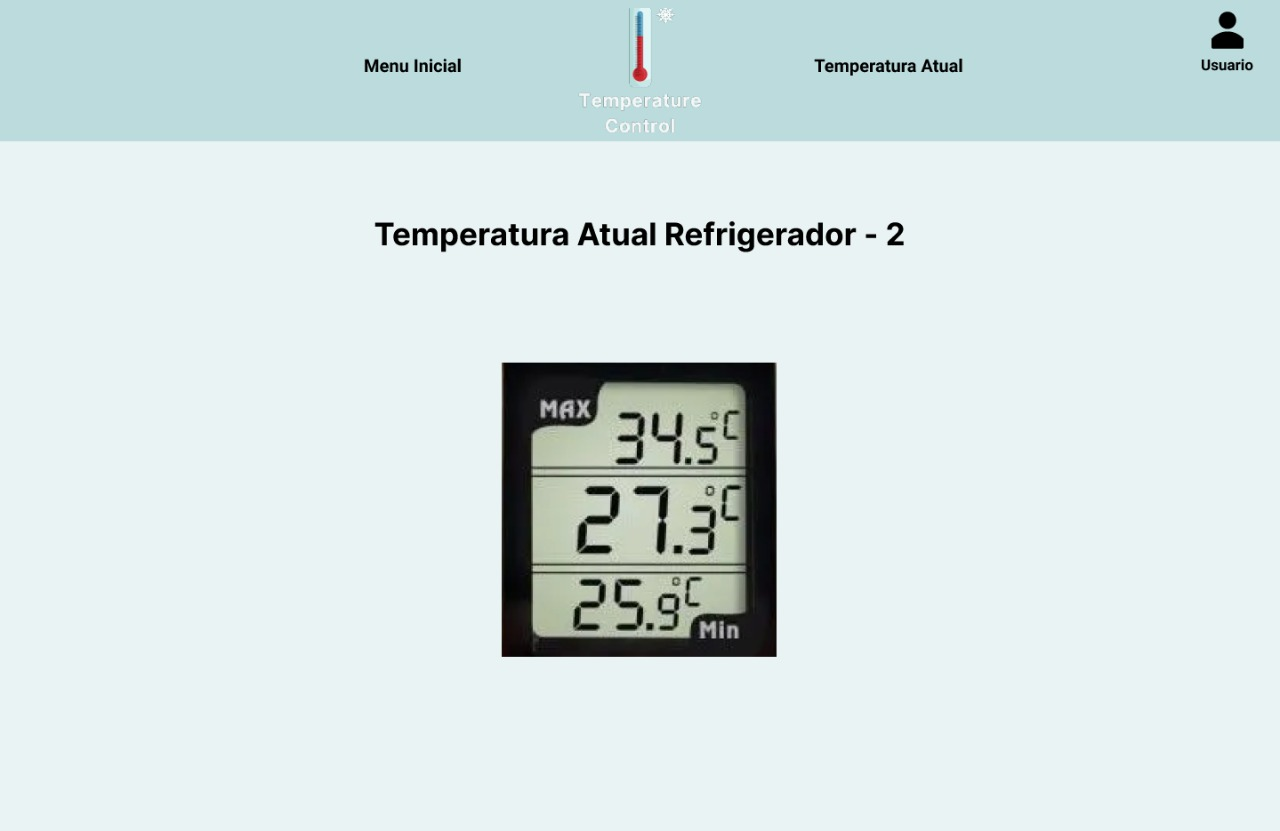
\includegraphics[scale=0.35]{img/desktop/temp_atual.jpeg}
        \legend{Fonte: Elaborado pelos autores}
        \label{fig:desktopTempAtual}
    \end{figure}
    \begin{figure}
        \caption{Layout desktop dashboard 1}
        \centering
        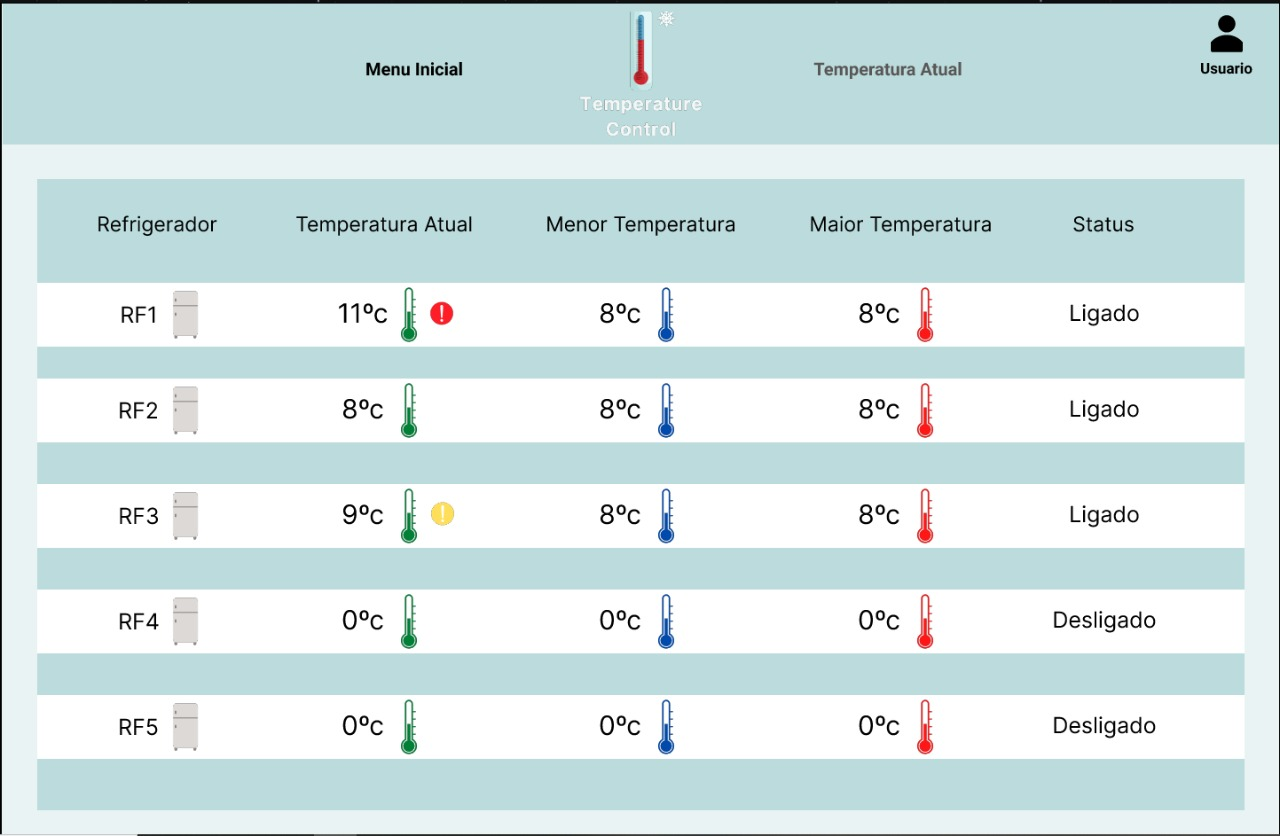
\includegraphics[scale=0.35]{img/desktop/dashboard_1.jpeg}
        \legend{Fonte: Elaborado pelos autores}
        \label{fig:desktopDashboard1}
    \end{figure}
    \begin{figure}
        \caption{Layout desktop dashboard 2}
        \centering
        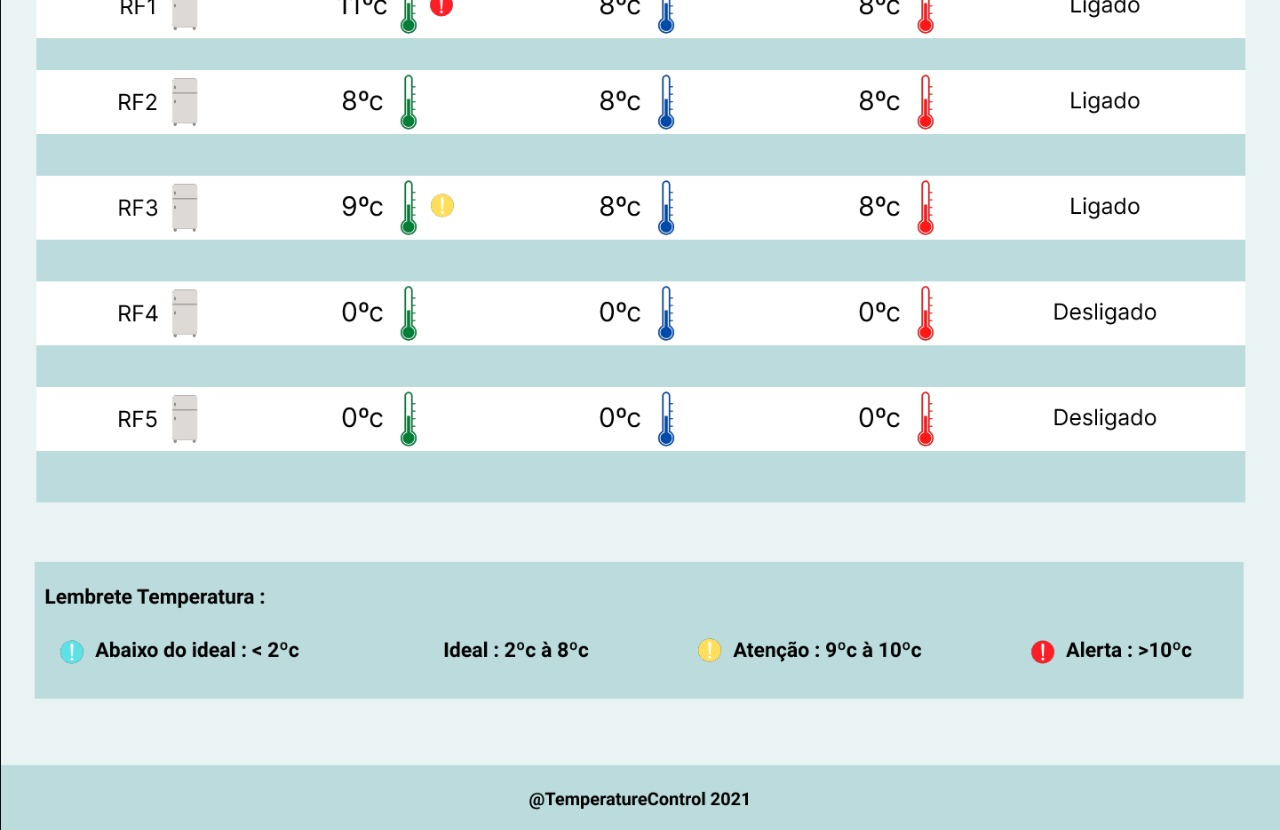
\includegraphics[scale=0.35]{img/desktop/dashboard_2.jpeg}
        \legend{Fonte: Elaborado pelos autores}
        \label{fig:desktopDashboard2}
    \end{figure}
    \begin{figure}
        \caption{Layout desktop histórico diário}
        \centering
        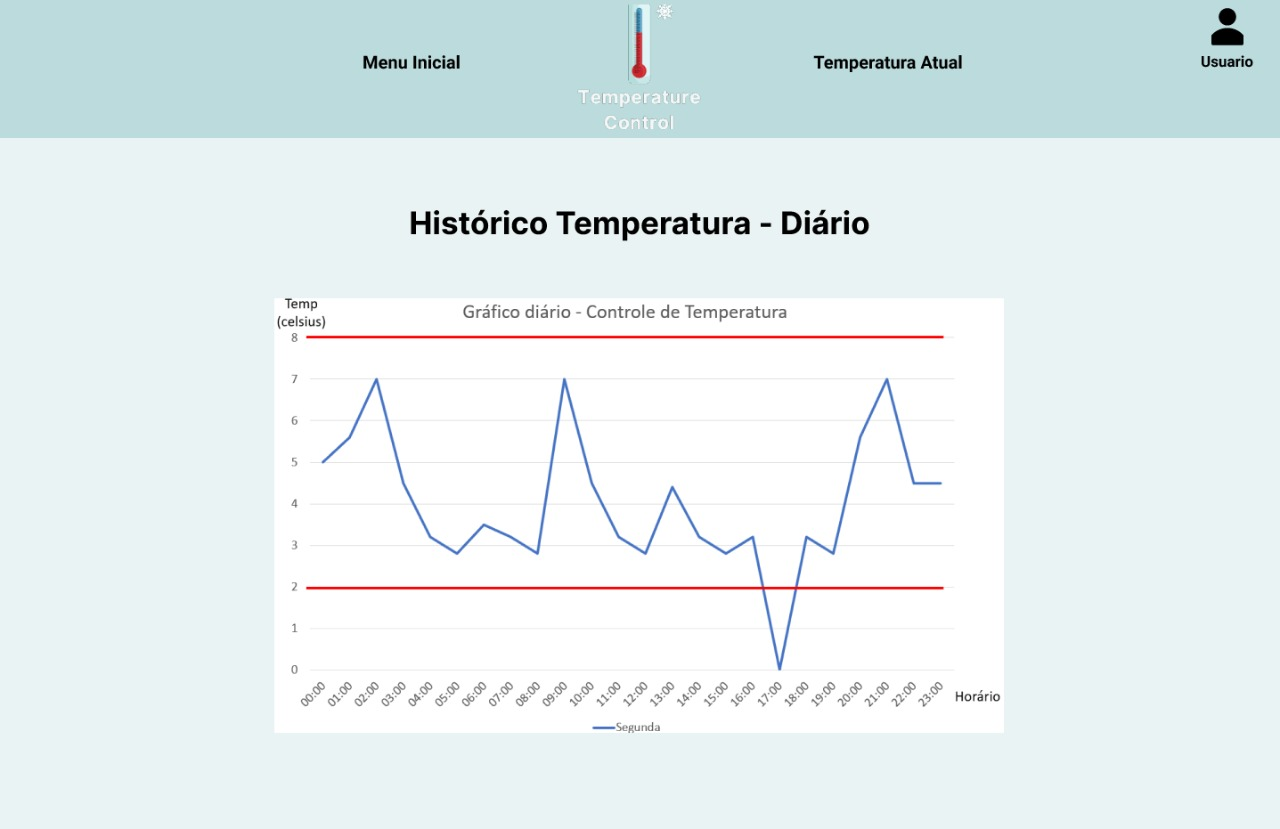
\includegraphics[scale=0.35]{img/desktop/temp_diaria.jpeg}
        \legend{Fonte: Elaborado pelos autores}
        \label{fig:desktopTempDiaria}
    \end{figure}
    \begin{figure}
        \caption{Layout desktop histórico semanal}
        \centering
        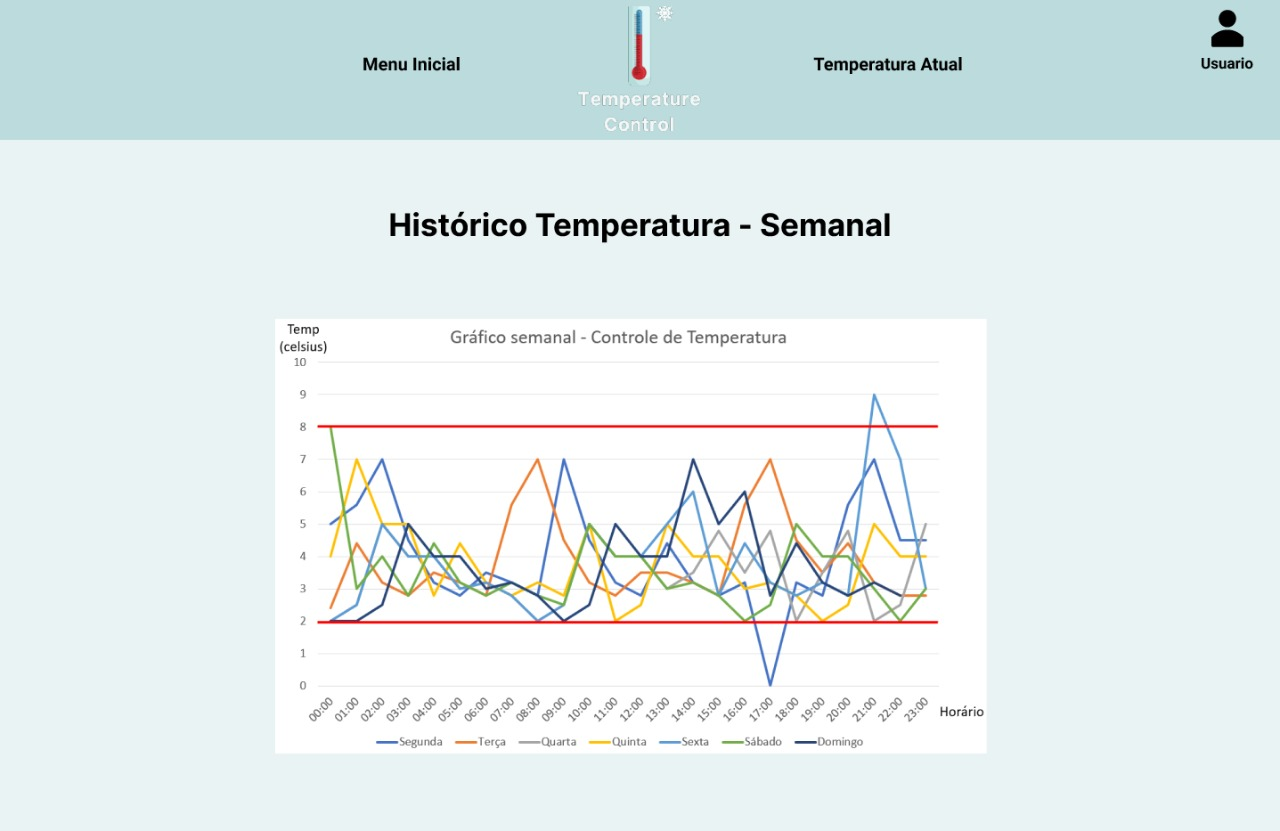
\includegraphics[scale=0.35]{img/desktop/temp_semanal.jpeg}
        \legend{Fonte: Elaborado pelos autores}
        \label{fig:desktopTempSemanal}
    \end{figure}


    \newpage

    Quanto a versão mobile do software,
    ela segue o mesmo padrão da versão desktop 
    possuindo as mesmas telas e funcionalidades,
    porem de forma a se adaptar melhor a telas 
    pequenas.


    \begin{figure}
        \centering
        \begin{minipage}{0.5\textwidth}
            \caption{Layout mobile Bem vindo}
            \centering
            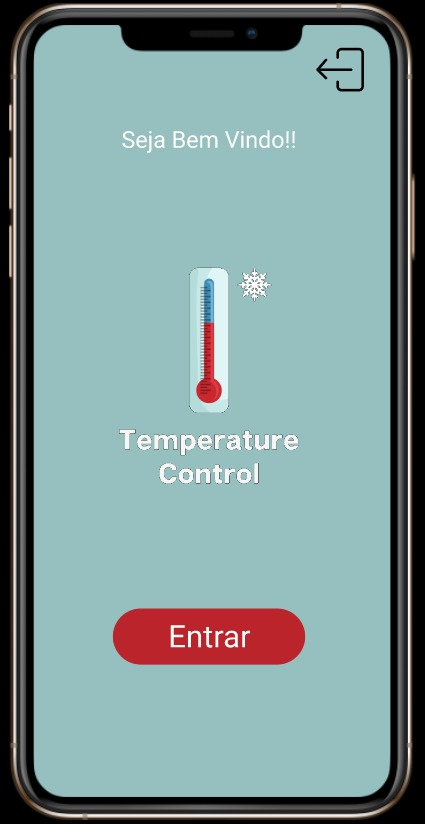
\includegraphics[height=0.4\textheight]{img/mobile/bem_vindo.png}
            \legend{Fonte: Elaborado pelos autores}
            \label{fig:mobileBemVindo}
        \end{minipage}%
        \begin{minipage}{0.5\textwidth}
            \caption{Layout mobile Home}
            \centering
            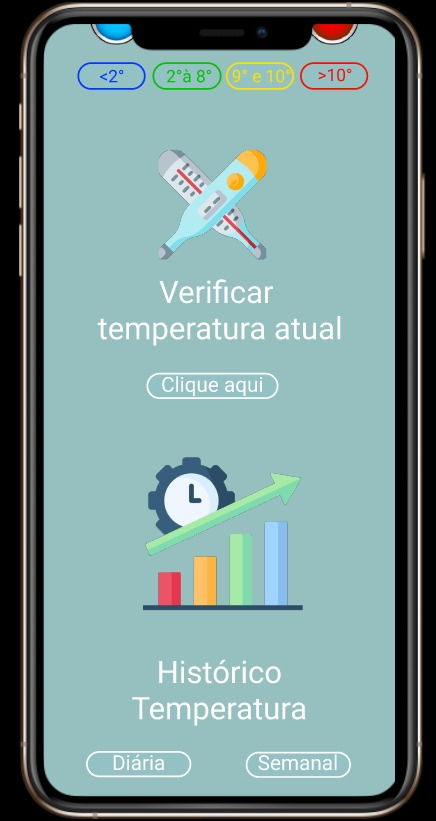
\includegraphics[height=0.4\textheight]{img/mobile/home.jpeg}
            \legend{Fonte: Elaborado pelos autores}
            \label{fig:mobileHome}
        \end{minipage}
    \end{figure}

    \begin{figure}
        \centering
        \begin{minipage}{0.5\textwidth}
            \caption{Layout mobile \\ configuração temperaturas}
            \centering
            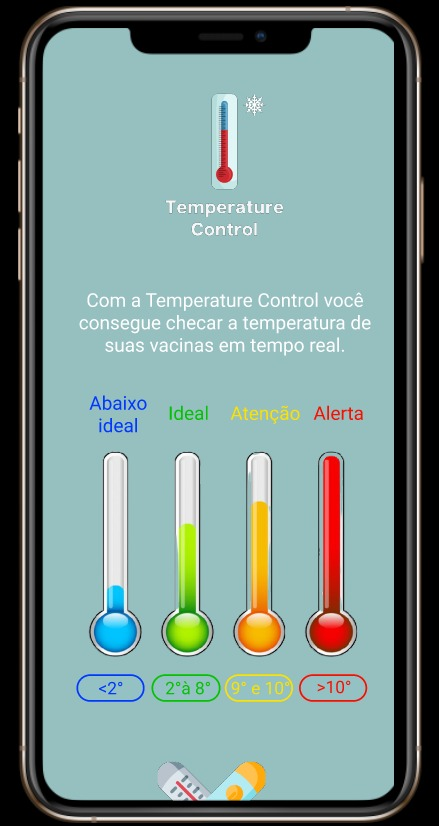
\includegraphics[height=0.4\textheight]{img/mobile/config_temp.jpeg}
            \legend{Fonte: Elaborado pelos autores}
            \label{fig:mobileConfig}
        \end{minipage}%
        \begin{minipage}{0.5\textwidth}
            \caption{Layout mobile \\ dashboard 1}
            \centering
            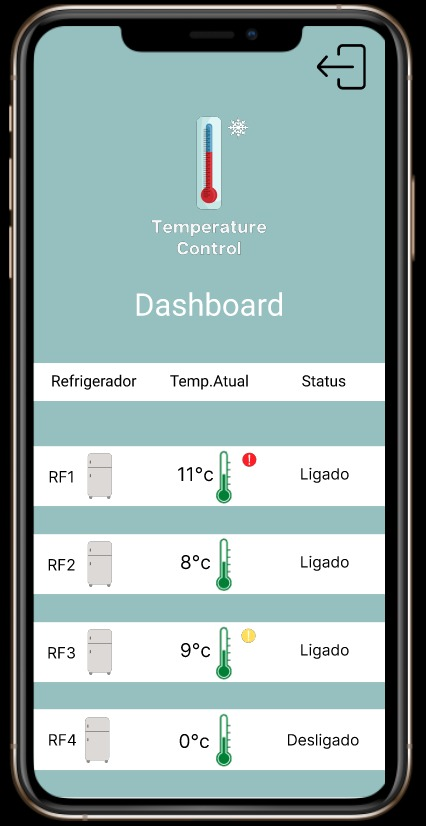
\includegraphics[height=0.4\textheight]{img/mobile/dashboard_1.jpeg}
            \legend{Fonte: Elaborado pelos autores}
            \label{fig:mobileDashboard1}
        \end{minipage}
    \end{figure}

    \begin{figure}
        \centering
        \begin{minipage}{0.5\textwidth}
            \caption{Layout mobile \\ dashboard 2}
            \centering
            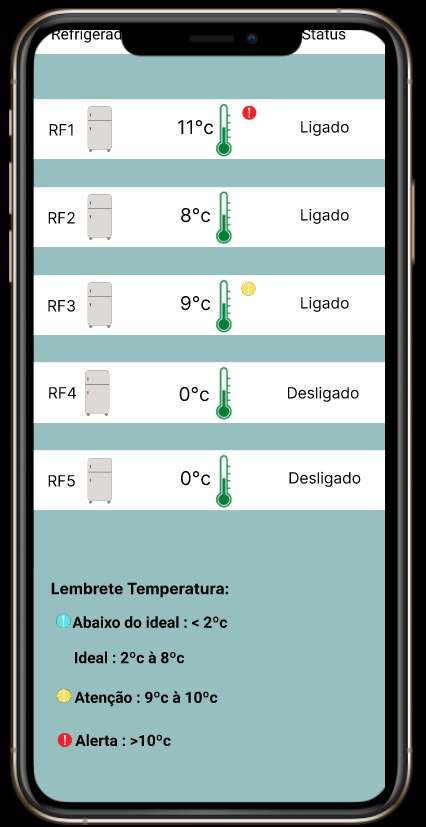
\includegraphics[height=0.4\textheight]{img/mobile/dashboard_2.jpeg}
            \legend{Fonte: Elaborado pelos autores}
            \label{fig:mobileDashboard2}
        \end{minipage}%
        \begin{minipage}{0.5\textwidth}
            \caption{Layout mobile \\ temperatura atual}
            \centering
            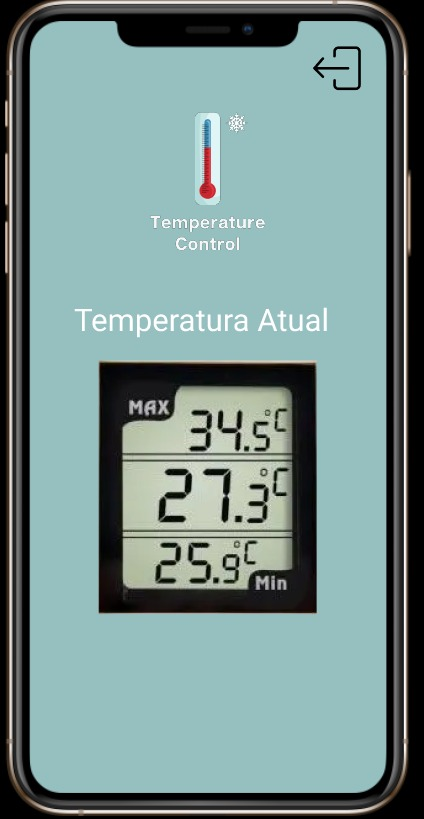
\includegraphics[height=0.4\textheight]{img/mobile/temp_atual.jpeg}
            \legend{Fonte: Elaborado pelos autores}
            \label{fig:mobileTempAtual}
        \end{minipage}
    \end{figure}

    \begin{figure}
        \begin{minipage}{0.5\textwidth}
            \caption{Layout mobile histórico diário}
            \centering
            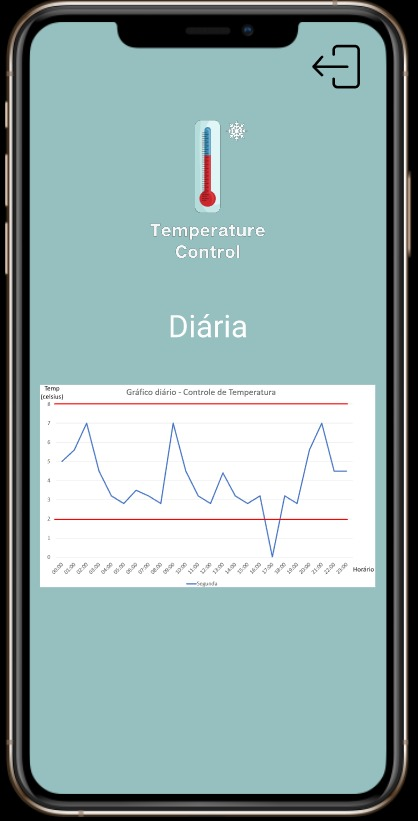
\includegraphics[height=0.4\textheight]{img/mobile/temp_diaria.jpeg}
            \legend{Fonte: Elaborado pelos autores}
            \label{fig:mobileTempDiaria}
        \end{minipage}%
        \begin{minipage}{0.5\textwidth}
            \caption{Layout mobile histórico semanal}
            \centering
            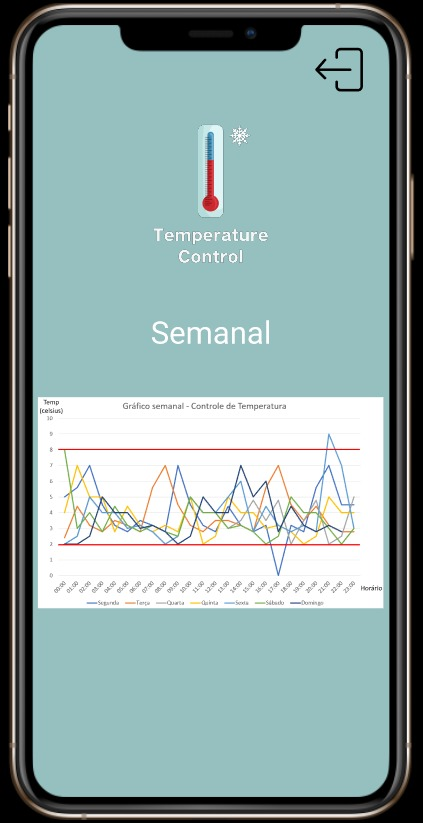
\includegraphics[height=0.4\textheight]{img/mobile/temp_semanal.jpeg}
            \legend{Fonte: Elaborado pelos autores}
            \label{fig:mobileTempSemanal}
        \end{minipage}
    \end{figure}

